There are two major phases in any ``Program Understanding'' tool: \textit{data collection} and \textit{data analysis}.
%
To understand the runtime behavior of applications, an efficient tracing mechanism is required to collect informative data during execution of the application.
%
Upon failure or observing unexpected behavior of the program (e.g., wrong answer), studying collected execution data would reveal insight about how program dynamically behaved and what went wrong.
%
In this section, we explain our methodology of data collection and data analysis towards debugging and locating potential root causes of unexpected behavior.
%
The main source of whole-program dynamic behavior is provided by ParLOT, a dynamic binary tracing tool that captures all function calls and returns and compress them on the fly (section \ref{subsec:parlot}).
%
After pre-processing ParLOT traces, a loop-detection-based lossless data reduction mechanism applies to each trace to
simplify collected data and reflect facts about loop structures (section \ref{subsec:nlr}).
%
Whole-program analysis in HPC applications only makes sense when the analysis includes cross-thread and cross-process as well as analysis of sequential control flow of every single running thread.
%
Inspired by many works\cite{weberStructural} \cite{Alqadah2011} \cite{Ignatov17}\cite{latticeForDistConst}, we have used FCA\cite{clbook} to integrate collected data into a single data structure as a whole, and extract valuable information about different aspect of the execution (section \ref{subsec:fca})
%
The major advantage of FCA, is that we can extract a full pair-wise similarity score matrix for all traces of a single execution in an efficient and scalable way, based on attributes that we extract from pre-processed traces.
%
Relying on similarities of traces, we classify traces (i.e., threads) into equivalent-behavior groups.
%
This way we reduce the search space from thousands of long traces to just a few classes of simplified trace representation
%
Any abnormal behavior of a thread (e.g., outlier) or group of threads can be detected (section \ref{subsec:exptmet}),
%
and for more-in-depth analysis, any pair of traces can be studied with respect to their entry orders and differences using a visualization (section \ref{subsec:diffnlr}).
%
\\
Section \ref{subsec:addrem} discusses some additional remarks (limitations, effectiveness of our approach)
\\
%

%TODO: The story builds on powerful components we have created.

% Binary tracing
\subsection{ParLOT: Efficient Trace Collection}
\label{subsec:parlot}

The final executable of real HPC applications are often a production of a large code base and a complex build system with numerous dependencies and libraries. Injecting instrumentation code to the source code, as in traditional tools like [????], is not feasible in HPC space. Also recompilation of the application with tools` compile-wrappers, as in TAU\cite{tau} and Score-p\cite{scorep}, may break the build system.
Also instrumentation and tracing mechanism of existing tools are often dependent to other libraries that are need to be present on the supercomputer for trace collection. [[ Example: STAT\cite{stat} and AutomaDeD\cite{automaded-laguna} that requires Dyninst\cite{dyninst} for instrumentation and MRNet\cite{mrnet} and TBON \cite{tbon}]]
%
To overcome the trade-off of comprehensive data collection while adding low time and space overhead, HPC program analysis tools often sacrifice one for the other. However, ParLOT collects whole-program function call traces at as low as library level, while incrementally compressing traces on-the-fly and leave majority of the system bandwidth for the application.
%
ParLOT collects \textit{whole} program function call traces with the mindset of \textit{paying a little upfront and save resource and time cost of reproducing the bug}.
%
ParLOT instruments the entry and exit point of each function in the binary using Pin\cite{pin} (fig. \ref{fig.parlotOverview}). Each ParLOT Trace contain full sequence of function calls and returns for every single thread that running the application code, reflecting the dynamic control flow and call-stack of the application individually.
%
Here we define ParLOT Trace, as we refer to it in the paper:

\begin{definition}{ParLOT Trace (PT)}
A ParLOT Trace $(PT)$ is a sequence of ordered integers $<f_i,...,f_j>$ where $f_0$ is \textit{return} and $f_k$ is the id of \textit{function k} ($k!=0$).
\end{definition}
%
Note that the $PT$ is the pre-processed (decompressed and filtered) version of immediate ParLOT traces. The fresh output of ParLOT traces are highly compressed byte-codes.
%
Also Note that $PT_{p.t}$ refers to the $PT$ that belongs to process $p$ and thread $t$ of that process.
%
\begin{figure}[t]
\caption{ParLOT Overview}
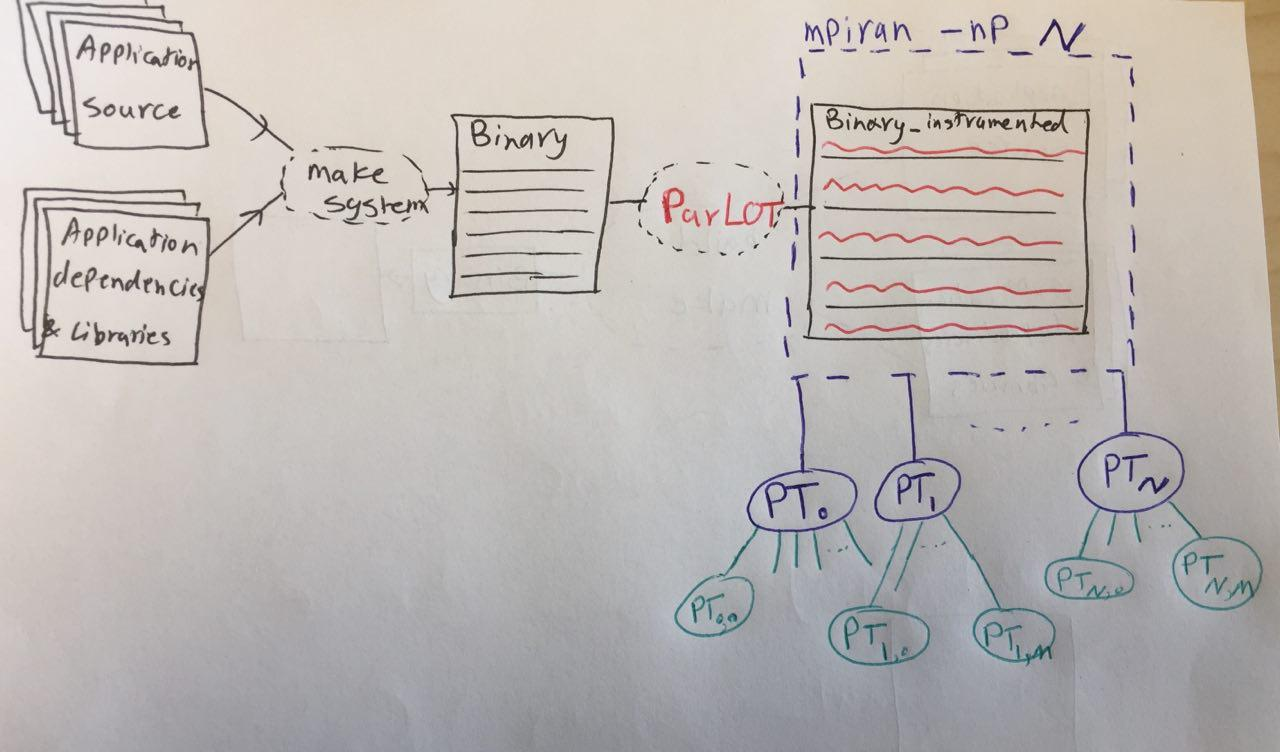
\includegraphics[width=0.45\textwidth]{figs/parlotOverview.jpg}
\label{fig.parlotOverview}
\end{figure}



% NLRs
\subsection{Loop structure detection}
\label{subsec:nlr}

HPC applications and resources are in interest of scientists and engineers for simulating \textit{iterative} kernels. Computer simulation of fluid dynamics, partial differential equations, Gauss-Seidel method and finite element methods in form of stencil codes do include a main outer loop that iterates over some elements (i.e., timesteps) and updates elements.
%
This character of typical HPC applications make PT lengths too long (millions) with much smaller number (hundreds) of distinct elements  (i.e., function IDs).
%
We propose a representation of PT elements (intra-PT compression) in form of \textit{loop structures}, such that PT = sequence of repetitive patterns (i.e, loops). In other words, each PT is a sequence of \textit{Loop Bodies (LB)} that repeated \textit{Loop Count (LC)} times, consecutively.
%


\subsubsection{Loops definition}

According to Makoto Kobayashi\cite{kobayashi-84} definition of loops, an occurrence of a \textit{loop} is defined as \textit{a sequence of elements} in which a particular sequence of \textit{distinct elements} (called the \textit{cycle} of the loop) is successively repeated.
%
Later Alain Ketterlin in \cite{Ketterlin-nlr} expanded this definition to numerical values for compressing and predicting memory access addresses and designed Nested Loop Recognition (NLR) algorithm.
%
The basic idea behind NLR algorithm is that a linear function model can be extracted from the linear progression in a sequence of numbers and these linear functions form a tree in which depth of each node is the depth of \textit{nested} loop(e.g., most outer loop's function is the root of the tree with depth 0).
%
We have modified NLR algorithm to make it suitable for PTs.
%
Each repetitive pattern and its frequency of consecutive appearances would be compressed to a single \textit{Loop Structure (LS)} entry.
%
\begin{definition}{Loop Structure} $LS = LB \; \hat{} \; LC$ where $LB  = <pt_i,...,pt_j>$ ($0<= i < j < len(PT)$) that occur $LC$ times is in a sub-sequence $ <pt_i,...,pt_k>$($k = 3j, k<len(PT)$)

\end{definition}
%
By converting each PT to a sequence of $LS_i$ , we reduce the length of PT by a factor of $\sum_i len(LB_i) * LC_i$.
%
Later we will explain how this lossless representation of PTs eases the process of diffing between a pair of PTs.

% CLs
\subsection{Equivalencing behavior via FCA}
\label{subsec:fca}
To Reduce the search space from thousands of PTs to just a few groups of equivalent PTs (i.e., inter-PT compression) not only requires a similarity measure based on a call matrix, but also requires a scheme that is efficient even for large process counts.
%
Since a pair-wise comparison of all processes is highly inefficient, we use \textit{concept lattices} that stem from \textit{formal concept analysis}(FCA)\cite{clbook} to store and compute groups of similar PTs.
%
A concept lattice is based on a \textit{formal context}\cite{clbook}, which is a triple $(O, A, I)$, where $O$ is a set of \textbf{objects}, $A$ a set of \textbf{attributes}, and $I \subseteq O \times A$ an incidence relation. The incidence relation associates each object with a set of attributes.
%
Due to its valuable properties,especially its \textit{partial order}, FCA has been used widely in computer science fields from machine learning and data mining \cite{Ignatov17} to distributed systems \cite{latticeForDistConst}.
%
However, since we are only interested in grouping similar PTs in this work, we only take advantage of similarity measures \cite{Alqadah2011} of concept lattices,
%
and left rest of its properties for our future work.
%
Due to typical HPC application common topologies such as SPMD, master/worker and odd/even where multiple processes/threads behave similarly, our experiments show that large number of PTs can be reduced to just a few groups.
%

\begin{frame}{}
  \lstset{language=C}
 \begin{lstlisting}
main(){
 int rank;
 int src;
 MPI_Init()
 MPI_Comm_size(MPI_COMM_WORLD)
 MPI_Comm_rank(MPI_COMM_WORLD,&rank)
 if (rank != 0) {
  MPI_Send(0) // Send to rank 0
 } else{ /* rank = 0
  MPI_Recv(1) // Receive from rank 1
  MPI_Recv(2) // Receive from rank 2
  MPI_Recv(3) // Receive from rank 3
 }
 MPI_Finalize()
}
\end{lstlisting}
\end{frame}



\begin{table}[]
\label{tab:sampleContext}
\caption{Context}
\scalebox{0.6}{
\begin{tabular}{l|cccccc}
 & \multicolumn{1}{l}{MPI\_Init()} & \multicolumn{1}{l}{MPI\_Comm\_Size()} & \multicolumn{1}{l}{MPI\_Comm\_Rank()} & \multicolumn{1}{l}{MPI\_Send()} & \multicolumn{1}{l}{MPI\_Recv()} & \multicolumn{1}{l}{MPI\_Finalize()} \\ \hline
Rank 0 & $\times$ & $\times$ & $\times$ &  & $\times$ & $\times$ \\
Rank 1 & $\times$ & $\times$ & $\times$ & $\times$ &  & $\times$ \\
Rank 2 & $\times$ & $\times$ & $\times$ & $\times$ &  & $\times$ \\
Rank 3 & $\times$ & $\times$ & $\times$ & $\times$ &  & $\times$
\end{tabular}}
\end{table}

\begin{figure}[t]
\centering
\scalebox{0.5}{
\includegraphics[width=3.4in]{figs/{sample}.pdf}}
\caption{Sample Concept Lattice from Obj-Atr Context in table\ref{tab:sampleContext}}

\label{fig:sampleCL}
\end{figure}

\begin{figure}[t]
\centering
\scalebox{0.5}{
\includegraphics[width=3.4in]{figs/{sample-reduced}.pdf}}
\caption{Concept Lattice with reduced labels}
\label{fig:sampleCL}
\end{figure}


\begin{figure}[t]
\centering
\scalebox{0.8}{
\includegraphics[width=3.4in]{figs/{fancy1}.pdf}}
\caption{Pair-wise Jaccard Similarity Matrix (JSM) of MPI processes in Sample code}
\label{fig:jsm}
\end{figure}

An example with
\\
- Source code [done]
\\
- Simple attributes and Context [done]
\\
- Concept Lattice [done]
\\
- Jaccard Similarity (heatmap or matrix) [done]
\\
- How we obtained JSM elements
\\
- Visualization of LCA [not yet]
\\
- CL construction \cite{clconst} \cite{bender05}
\\
- Attribute Table


\subsection{diffNLR: Reflecting differences}
\label{subsec:diffnlr}
-From fig we can see that PT0 and PT1 are in different groups with similarity of XX.
%
\\
Inspired by \texttt{diff} original algorithm\cite{diff-myers} that has bin used in Git and GNU Diff, we visualize the differences of a pair of PT as shown in fig \ref{fig:sampleDiffNLR}.
\\
This visualization reflects of the differences of \textbf{occurrences} of PT elements and their \textbf{orders}.
\\
In section \ref{sec:experimental} we show how this visualization can help us locating the points of divergence in PTs, and potential bug manifestation and root cause.

\begin{figure}[t]
\centering
\scalebox{0.5}{
\includegraphics[width=3.4in]{figs/{sampleDiffNLR}.png}}
\caption{Sample diffNLR}
\label{fig:sampleDiffNLR}
\end{figure}

\subsection{Experimental Methodology}
\label{subsec:exptmet}

- Candidates to look at and observe their diffNLR: $(PT_i, PT_j) = Max | JSM[i][j](buggy) - JSM[i][j](bugfree)| $

- It means the similarity of $(PT_i, PT_j)$ of buggy execution have the highest difference with its corresponding similarity of the bug-free execution.

- Figures are showing two \textit{diffNLR} side by side, one is $diffNLR(i,j)_{buggy}$ and the other one is  $diffNLR(i,j)_{bugfree}$ where $i, j$ obtained from candidate tables.

- Two additional tables that show the LB (loop body) of each detected loop. $L_i$

\subsection{Additional Remarks}
\label{subsec:addrem}
